\textbf{Problem 1.}

The $p$-norm of a vector $\underline{v}\in\mathbb{R}^n$ is defined as
\begin{align*}
    \norm{\underline{v}}_p = \left( \sum_{i=1}^n \abs{v_i}^p \right)^{1/p}
\end{align*}

\begin{enumerate}[label=(\roman*),leftmargin=*,itemsep=0mm]
    
    \item We draw the region in the $xy$-plane where $\norm{v}_p\leq1$ when $\underline{v}=(x,y)$ for $p=1,2,\infty$:
    
    \begin{figure*}[h!]
    \centering
    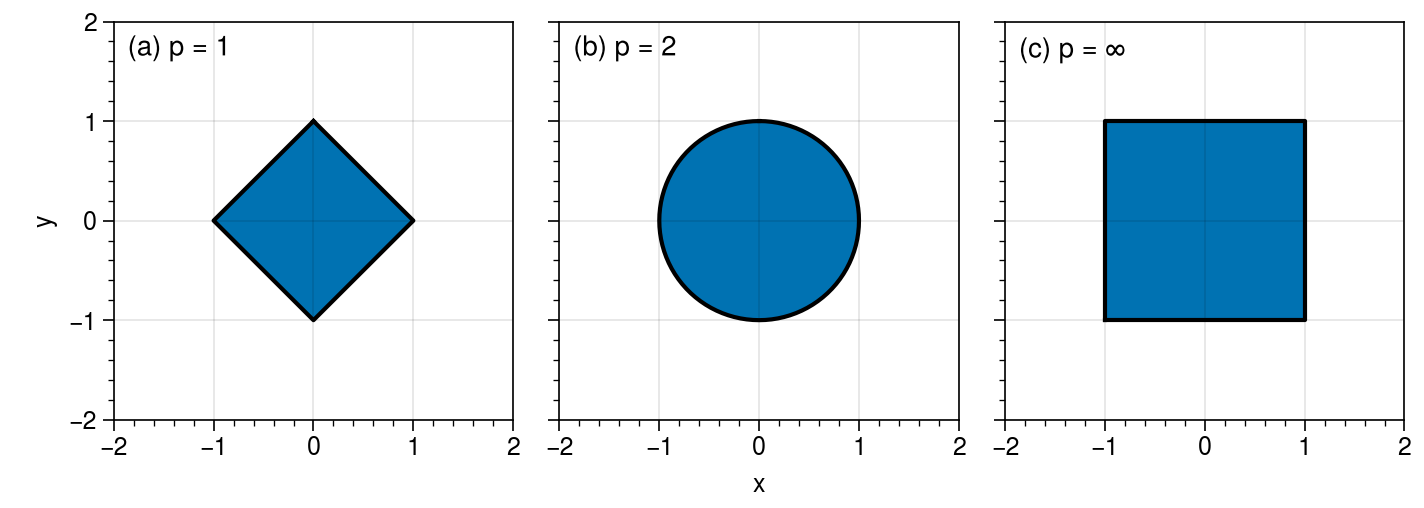
\includegraphics[width=0.9\textwidth]{figures/hw2_qn1.png}\\
    \caption{}
    \label{hw2_qn1}
    \end{figure*}
    
    \item The dual norm of $\norm{\cdot}_p$, $\norm{\cdot}_q$, is defined to be
    \begin{align*}
        \norm{\underline{v}}_q
        = \max_{\underline{w}} \frac{\underline{w}^T\underline{v}}{\norm{\underline{w}}_p}
        = \max_{\underline{w}}
        \{ \underline{w}^T\underline{v} : \norm{\underline{w}}_p=1 \}
        = \max \langle\underline{w}^T,v\rangle : \norm{\underline{w}}_p=1
    \end{align*}
    
    For $p=2$, we see that, given that $\underline{w}$ and $\underline{v}$ are vectors in the 2D space, with angle $\theta$ between them such that
    \begin{align*}
        \norm{\underline{v}}_q
        &= \max_{\underline{w}}
        \{ \underline{w}^T\underline{v} : \norm{\underline{w}}_p=1 \}
        = \max_{\underline{w}}
        \{ \norm{\underline{w}}_2 \norm{\underline{v}}_2 \cos\theta : \norm{\underline{w}}_p=1 \} \\
        &\leq \max_{\underline{w}}
        \{ \norm{\underline{w}}_2 \norm{\underline{v}}_2 : \norm{\underline{w}}_p=1 \} \\
        &= \norm{\underline{v}}_2
    \end{align*}
    
    Since it is a given that $\norm{\underline{w}}_2 = 1$.  Thus we have shown that the dual norm of $ \norm{\underline{v}}_2$ is $ \norm{\underline{v}}_2$.
    
    For $p=1$, we see that
    \begin{align*}
        \underline{w}^T\underline{v} 
        &= \sum_{i=1}^n w_iv_i 
        \leq \sum_{i=1}^n \abs{w_iv_i}
        \leq \sum_{i=1}^n \abs{w_i}\abs{v_i} \\
        &\leq \left( \max_{i=1}^n \abs{v_i} \right) \cdot \sum_{i=1}^n\abs{w_i}
        = \max_{i=1}^n \abs{v_i} \\
        &= \norm{\underline{v}}_\infty \\
        \therefore \norm{\underline{v}}_q
        &= \max_{\underline{w}} \frac{\underline{w}^T\underline{v}}{\norm{\underline{w}}_p}
        = \frac{\norm{\underline{v}}_\infty}{\norm{\underline{w}}_1}
        = \norm{\underline{v}}_\infty
    \end{align*}
    
    Similarly, for $p=\infty$
    \begin{align*}
        \underline{w}^T\underline{v} 
        &\leq \sum_{i=1}^n \abs{w_i}\abs{v_i}
        \leq \left( \max_{i=1}^n \abs{w_i} \right) \cdot \sum_{i=1}^n\abs{v_i} \\
        &= \norm{\underline{w}}_\infty \sum_{i=1}^n \abs{v_i} \\
        \therefore \norm{\underline{v}}_q
        &= \max_{\underline{w}} \frac{\underline{w}^T\underline{v}}{\norm{\underline{w}}_p}
        = \frac{\norm{\underline{w}}_\infty \sum_{i=1}^n \abs{v_i}}{\norm{\underline{w}}_\infty}
        = \sum_{i=1}^n \abs{v_i} \\
        &= \norm{\underline{v}}_1
    \end{align*}
    
\end{enumerate}